\documentclass[tikz,border=10pt]{standalone}
\usepackage[T1]{fontenc}
\usepackage{helvet}
\renewcommand{\familydefault}{\sfdefault}
\usepackage{tikz}
\usetikzlibrary{arrows.meta,positioning,shapes.multipart,shapes.geometric,fit,backgrounds,calc,shadows}

\definecolor{navy}{HTML}{1F3A5F}
\definecolor{teal}{HTML}{0C6B58}
\definecolor{amber}{HTML}{D9822B}
\definecolor{crimson}{HTML}{B42318}
\definecolor{violet}{HTML}{6B21A8}
\definecolor{sky}{HTML}{2186EB}
\definecolor{slate}{HTML}{486581}
\definecolor{mist}{HTML}{F0F4F8}
\definecolor{line}{HTML}{9FB3C8}

\tikzset{
  >={Stealth[length=2.6mm]},
  box/.style={draw=navy, very thick, rounded corners=3pt, fill=white, align=center,
    inner sep=5pt, font=\small, minimum height=9mm},
  softbox/.style={box, draw=slate, thick, fill=mist},
  layer/.style={draw=line, dashed, rounded corners=6pt, inner sep=7pt},
  layertitle/.style={font=\bfseries\small, text=slate, anchor=north west},
  flow/.style={->, thick, draw=navy},
  dflow/.style={->, thick, draw=slate, dashed},
  lbl/.style={font=\scriptsize, text=slate, fill=white, inner sep=1.5pt},
  umlclass/.style={draw=navy, thick, fill=white, rectangle split, rectangle split parts=3,
    rectangle split part fill={navy!12,white,white}, align=left, font=\scriptsize,
    inner sep=3pt, text width=#1},
  umlclass/.default=38mm,
}

\begin{document}
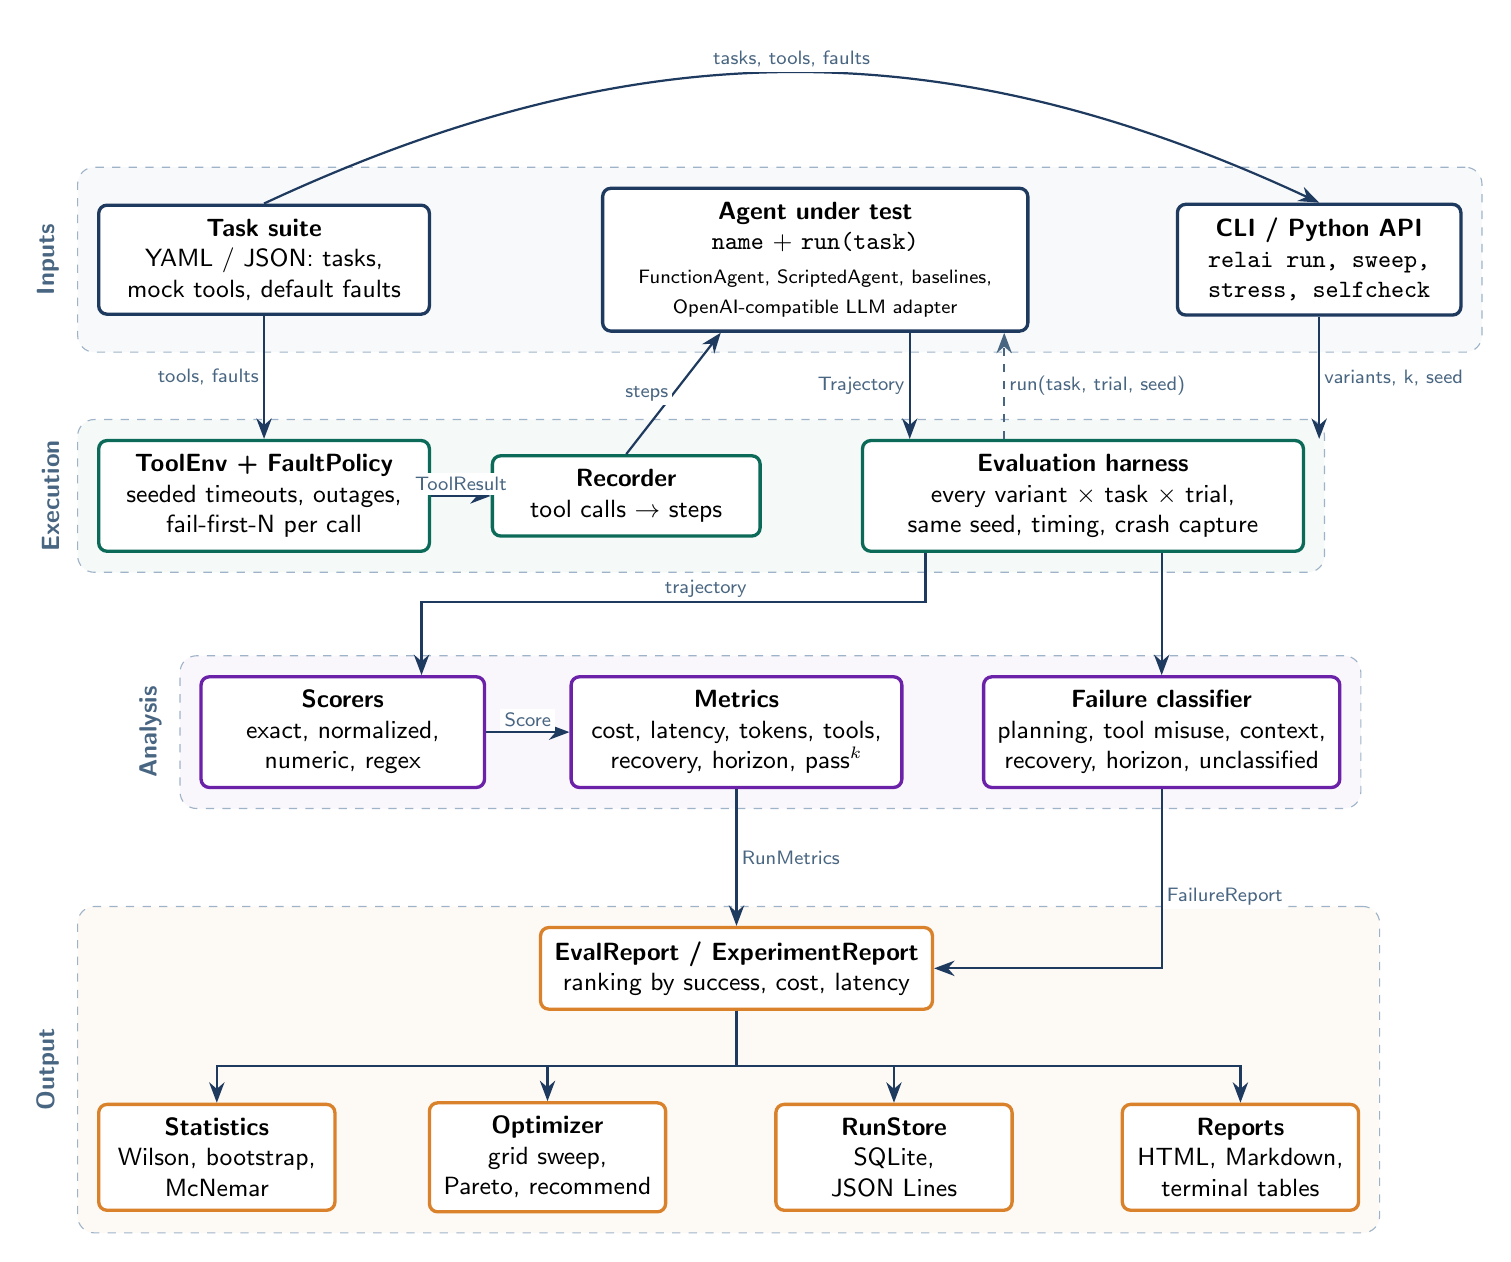
\begin{tikzpicture}[x=1cm,y=1cm]
  % Inputs
  \node[box, minimum width=4.2cm] (suite) at (0,0) {\textbf{Task suite}\\YAML / JSON: tasks,\\mock tools, default faults};
  \node[box, minimum width=5.4cm] (agents) at (7,0) {\textbf{Agent under test}\\\texttt{name} + \texttt{run(task)}\\[1pt]\scriptsize FunctionAgent, ScriptedAgent, baselines,\\\scriptsize OpenAI-compatible LLM adapter};
  \node[box, minimum width=3.6cm] (cli) at (13.4,0) {\textbf{CLI / Python API}\\\texttt{relai run, sweep,}\\\texttt{stress, selfcheck}};

  % Execution
  \node[box, draw=teal, minimum width=4.2cm] (env) at (0,-3) {\textbf{ToolEnv + FaultPolicy}\\seeded timeouts, outages,\\fail-first-N per call};
  \node[box, draw=teal, minimum width=3.4cm] (rec) at (4.6,-3) {\textbf{Recorder}\\tool calls $\rightarrow$ steps};
  \node[box, draw=teal, minimum width=5.6cm] (harness) at (10.4,-3) {\textbf{Evaluation harness}\\every variant $\times$ task $\times$ trial,\\same seed, timing, crash capture};

  % Analysis
  \node[box, draw=violet, minimum width=3.6cm] (scorer) at (1,-6) {\textbf{Scorers}\\exact, normalized,\\numeric, regex};
  \node[box, draw=violet, minimum width=4.2cm] (metrics) at (6,-6) {\textbf{Metrics}\\cost, latency, tokens, tools,\\recovery, horizon, pass$^k$};
  \node[box, draw=violet, minimum width=4.4cm] (classifier) at (11.4,-6) {\textbf{Failure classifier}\\planning, tool misuse, context,\\recovery, horizon, unclassified};

  % Outputs
  \node[box, draw=amber, minimum width=4.4cm] (report) at (6,-9) {\textbf{EvalReport / ExperimentReport}\\ranking by success, cost, latency};
  \node[box, draw=amber, minimum width=3.0cm] (stats) at (-0.6,-11.4) {\textbf{Statistics}\\Wilson, bootstrap,\\McNemar};
  \node[box, draw=amber, minimum width=3.0cm] (opt) at (3.6,-11.4) {\textbf{Optimizer}\\grid sweep,\\Pareto, recommend};
  \node[box, draw=amber, minimum width=3.0cm] (store) at (8.0,-11.4) {\textbf{RunStore}\\SQLite,\\JSON Lines};
  \node[box, draw=amber, minimum width=3.0cm] (html) at (12.4,-11.4) {\textbf{Reports}\\HTML, Markdown,\\terminal tables};

  % Layer frames with titles on the left edge
  \begin{scope}[on background layer]
    \node[layer, fit=(suite)(agents)(cli), fill=navy!3] (L1) {};
    \node[layer, fit=(env)(rec)(harness), fill=teal!4] (L2) {};
    \node[layer, fit=(scorer)(metrics)(classifier), fill=violet!4] (L3) {};
    \node[layer, fit=(report)(stats)(opt)(store)(html), fill=amber!5] (L4) {};
  \end{scope}
  \foreach \frame/\title in {L1/Inputs, L2/Execution, L3/Analysis, L4/Output} {
    \node[font=\bfseries\small, text=slate, rotate=90, anchor=south] at ([xshift=-3pt]\frame.west) {\title};
  }

  % Flows
  \draw[flow] (suite.north) to[out=25, in=155] node[lbl, pos=0.5, above] {tasks, tools, faults} (cli.north);
  \draw[flow] (suite) -- node[lbl, left] {tools, faults} (env);
  \draw[flow] (env) -- node[lbl, above] {ToolResult} (rec);
  \draw[flow] (rec.north) -- node[lbl, left] {steps} ([xshift=-12mm]agents.south);
  \draw[flow] ([xshift=12mm]agents.south) -- node[lbl, left] {Trajectory} ([xshift=12mm]agents.south |- harness.north);
  \draw[dflow] ([xshift=24mm]agents.south |- harness.north) -- node[lbl, right] {run(task, trial, seed)} ([xshift=24mm]agents.south);
  \draw[flow] (cli.south) -- node[lbl, right] {variants, k, seed} (cli.south |- harness.north);
  \draw[flow] ([xshift=-20mm]harness.south) |- node[lbl, pos=0.75, above] {trajectory} (scorer.east |- 0,-4.35) -- ++(0,0) -| ([xshift=10mm]scorer.north);
  \draw[flow] (scorer) -- node[lbl, above] {Score} (metrics);
  \draw[flow] ([xshift=10mm]harness.south) -- ([xshift=10mm]harness.south |- classifier.north);
  \draw[flow] (metrics) -- node[lbl, right] {RunMetrics} (report);
  \draw[flow] (classifier.south) |- node[lbl, pos=0.3, right] {FailureReport} (report.east);
  \draw[flow] (report.south) -- ++(0,-0.7) -| (stats.north);
  \draw[flow] (report.south) -- ++(0,-0.7) -| (opt.north);
  \draw[flow] (report.south) -- ++(0,-0.7) -| (store.north);
  \draw[flow] (report.south) -- ++(0,-0.7) -| (html.north);
\end{tikzpicture}
\end{document}
